\subsection{Ellipsoids in added-variable plots}\label{sec:avp}

In contrast to the marginal, bivariate views of the relationships of a response to several predictors (e.g., such as shown in the top row of the scatterplot matrix in \figref{fig:vis-reg-coffee11}), \emph{added-variable plots}
(aka \emph{partial regression plots}) show the partial relationship between the response and
each predictor, where the effects of all other predictors have been controlled or adjusted for.
Again we find that such plots have remarkable geometric properties, particularly
when supplemented by ellipsoids.

\begin{figure}[htb]
 \begin{minipage}[b]{.49\linewidth}
  \centering
  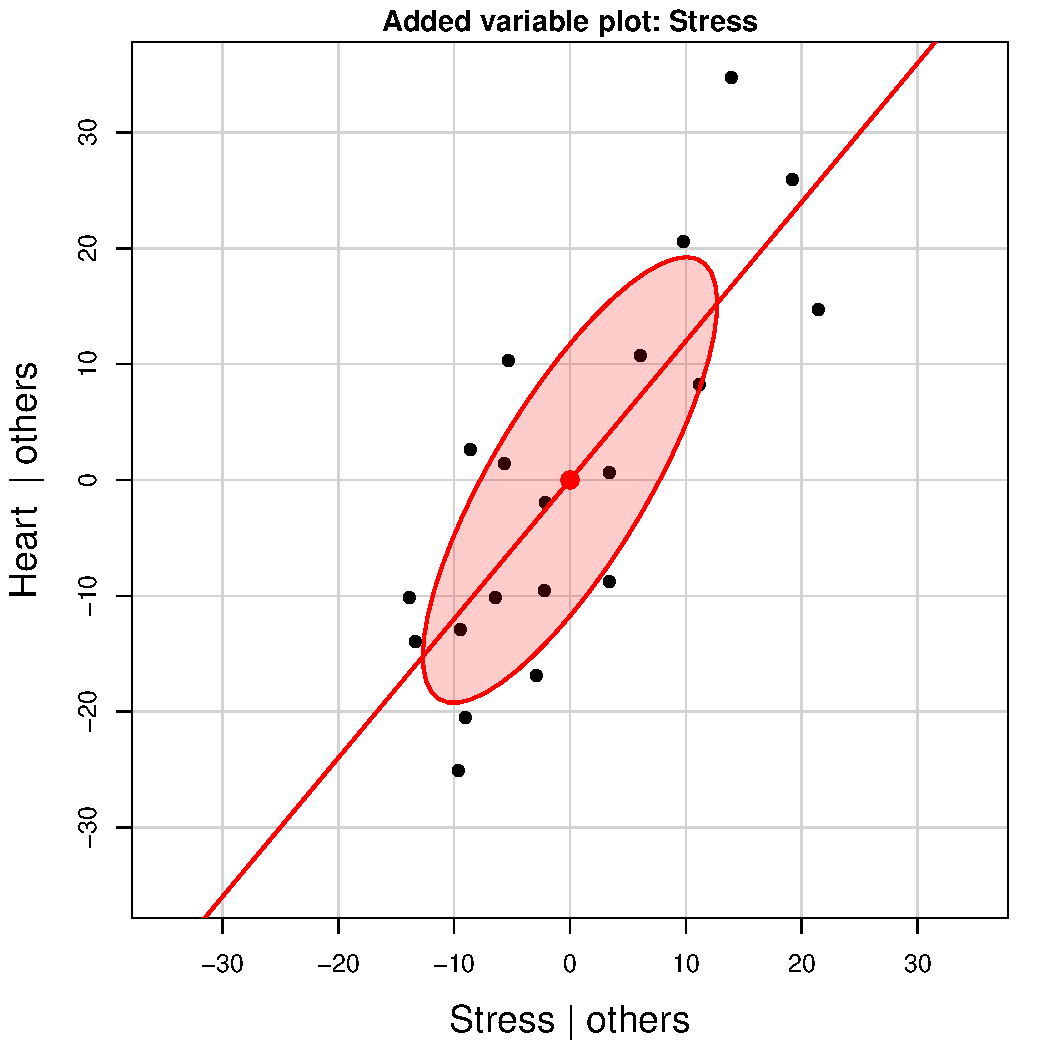
\includegraphics[width=1\linewidth]{fig/coffee-avplot1}
%  \caption{}%
%  \label{fig:}
 \end{minipage}%
 \hfill
 \begin{minipage}[b]{.49\linewidth}
  \centering
  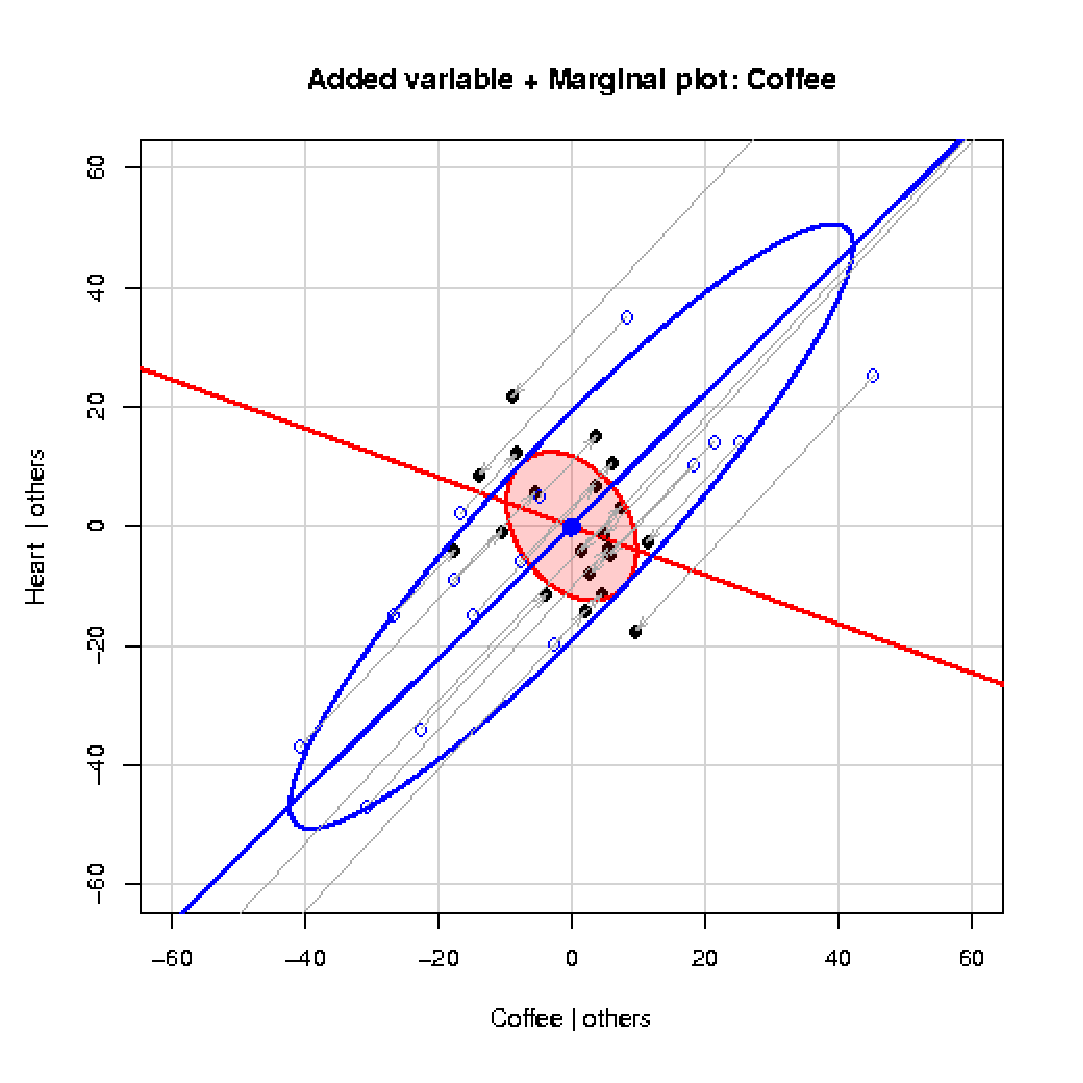
\includegraphics[width=1\linewidth]{fig/coffee-avplot2}
 \end{minipage}
  \caption{Added variable plots for Stress and Coffee in the multiple regression predicting Heart disease.
Each panel also shows the 50\% conditional data ellipse for residuals $(\vec{x}_k^\star, \vec{y}^\star)$, shaded red.
}
  \label{fig:coffee-avplot-A}
\end{figure}

Formally, we express the standard linear model in vector form as
$\widehat{\vec{y}} \equiv \widehat{\vec{y}} \given \mat{X} = \beta_0 \vec{1} + \beta_1 \vec{x}_1 + \beta_2 \vec{x}_2 + \dots +  \beta_p \vec{x}_p$,
with model matrix $\mat{X} = [ \vec{1}, \vec{x}_1, \dots \vec{x}_p ]$.
Let $\mat{X}_{[-k]}$ be the model matrix omitting the column for variable $k$.
Then algebraically, the added variable plot for variable $k$ is the scatterplot of the residuals $(\vec{x}^\star_k, \vec{y}^\star)$ from
two auxillary regressions, fitting $\vec{y}$ and $\vec{x}_k$ from $\mat{X}_{[-k]}$,
\begin{eqnarray*}
 \vec{y}^\star   & \equiv & \vec{y} \given \textrm{others}  =  \vec{y} - \widehat{\vec{y}} \given \mat{X}_{[-k]} \\
 \vec{x}^\star_k & \equiv & \vec{x}_k \given \textrm{others}  =  \vec{x}_k - \widehat{\vec{x}}_k \given \mat{X}_{[-k]}  \period \\
\end{eqnarray*}
(These quantities can all be computed \citep{VellemanWelsh:81} from the results of a single regression for the full model.)

Geometrically, in the space of the observations,\footnote{The ``space of the observations'' is yet a third, $n$-dimensional, space, in which the observations are the axes and each variable is represented as a point (or vector). See, e.g., \citet[Ch.~10]{Fox:2008}.} the fitted vector $\widehat{\vec{y}}$ is the orthogonal projection of $\vec{y}$
onto the subspace spanned by $\mat{X}$. Then $\vec{y}^\star$ and $\vec{x}^\star_k$ are the projections onto
the orthogonal complement of the subspace spanned by $\mat{X}_{[-k]}$, so
the simple regression of $\vec{y}^\star$ on $\vec{x}^\star_k$ has slope $\hat{\beta_k}$ in the full model,
and the residuals from the line $\vec{y}^\star = \hat{\beta_k} \vec{x}^\star_k$ in this plot are identically
the residuals from the overall regression of $\vec{y}$ on $\mat{X}$.

Another way to describe the added-variable plot (AVP) for $x_k$ is as a 2D projection of the space of
$(\vec{y}, \mat{X})$, viewed in the plane defined by the intersection of two hyperplanes:
the plane of the regression of $\vec{y}$ on all of $\mat{X}$, and the plane of regression of
$\vec{y}$ on $\mat{X}_{[-k]}$. A third plane, that of the regression of $x_k$ on $\mat{X}_{[-k]}$
also intersects in this space, and defines the horizontal axis in the AVP.
This is illustrated in \figref{fig:coffee-av3D}, showing one view defined by the intersection of
the three planes in the right panel.%
\footnote{Animated 3D movies of this plot are included among the supplementary materials for this paper.}

\begin{figure}[htb]
 \begin{minipage}[b]{.49\linewidth}
  \centering
  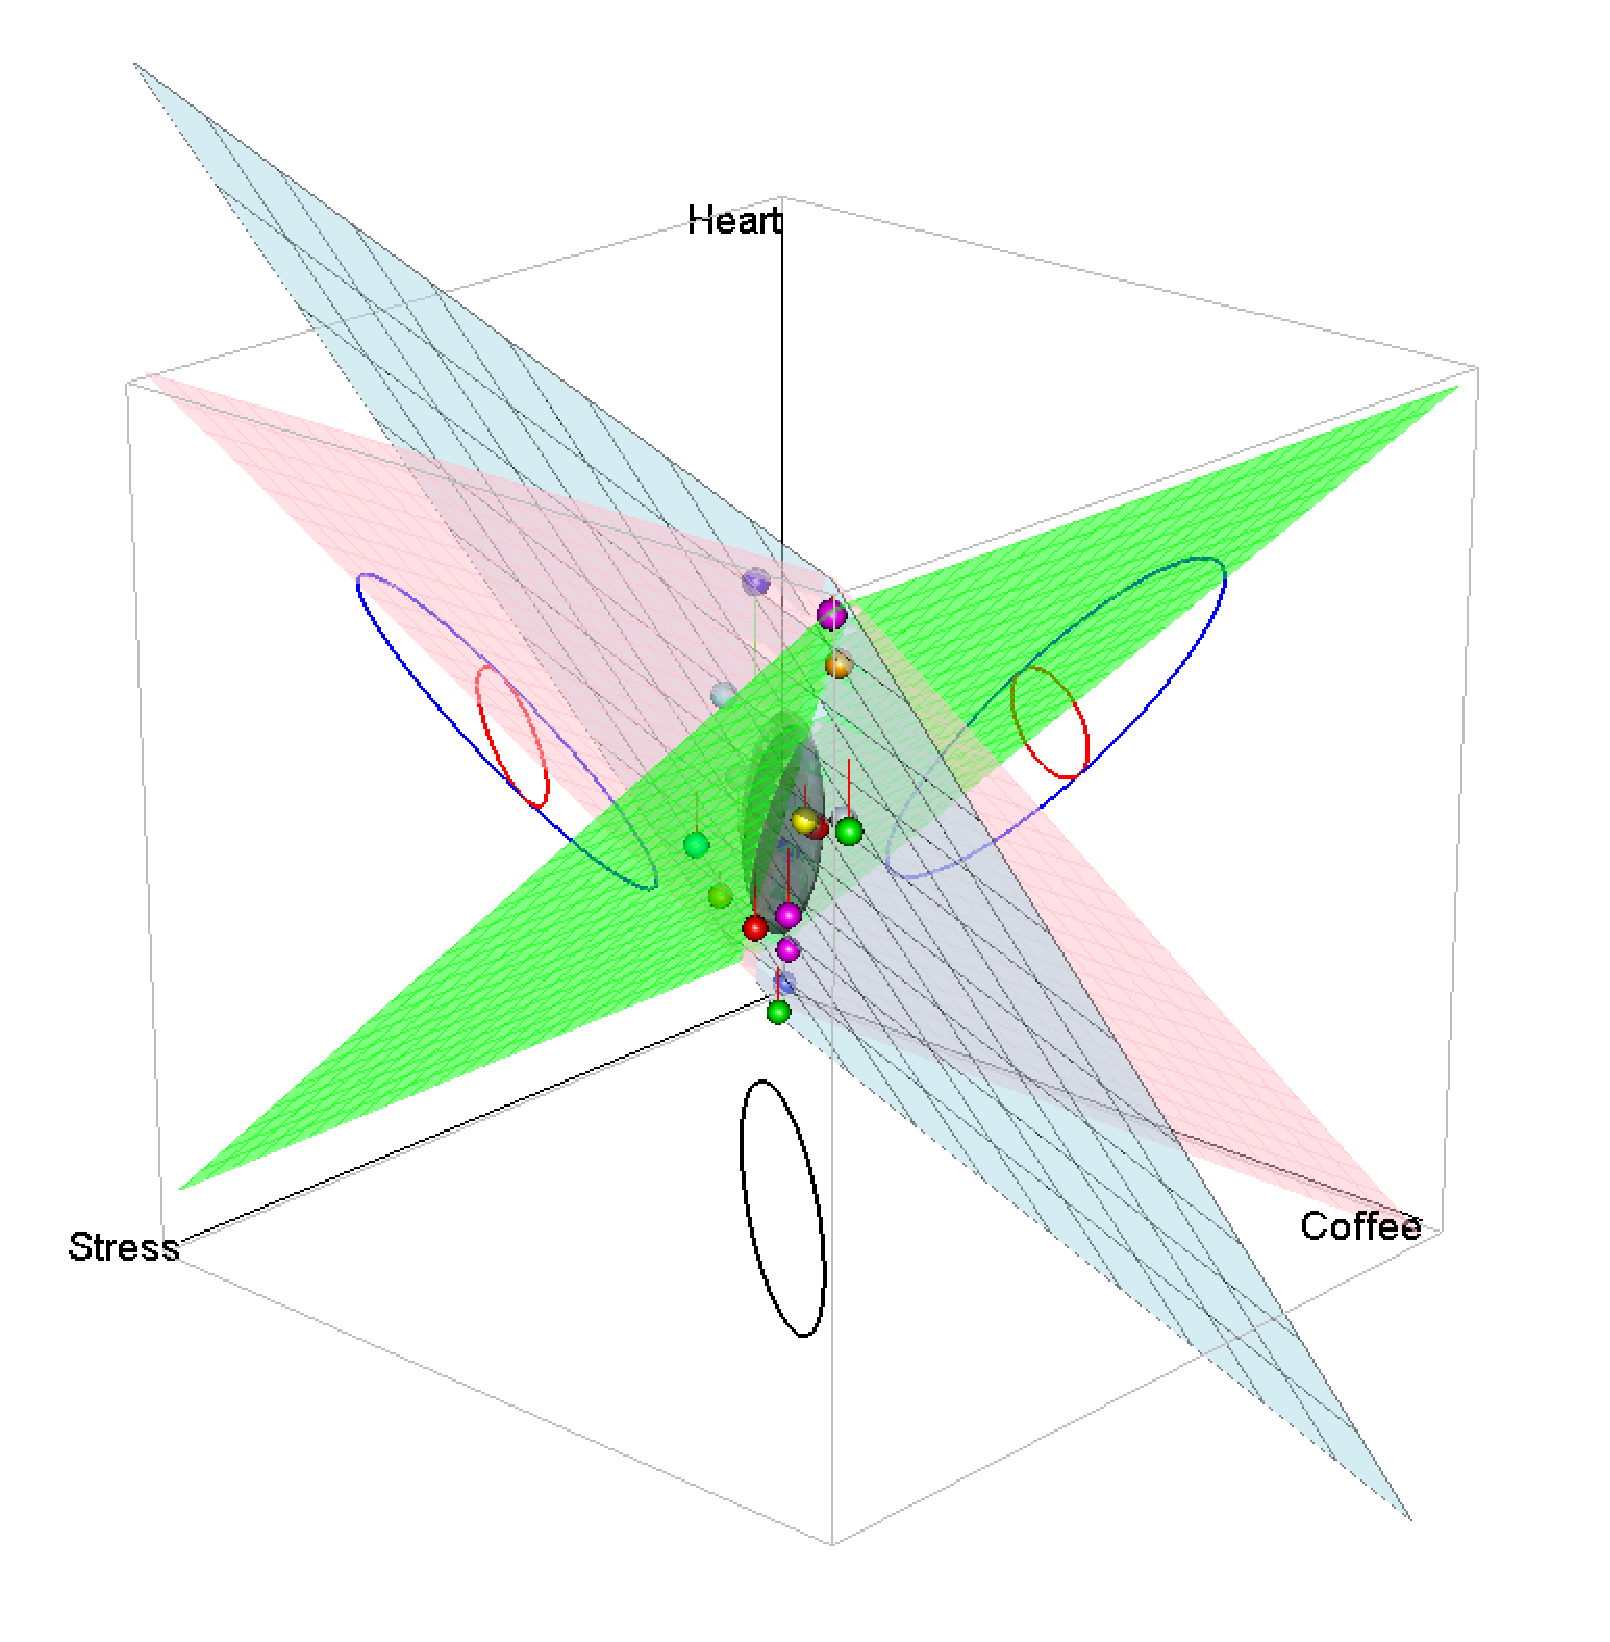
\includegraphics[width=1\linewidth]{fig/coffee-av3D-1}
%  \caption{}%
%  \label{fig:}
 \end{minipage}%
 \hfill
 \begin{minipage}[b]{.49\linewidth}
  \centering
  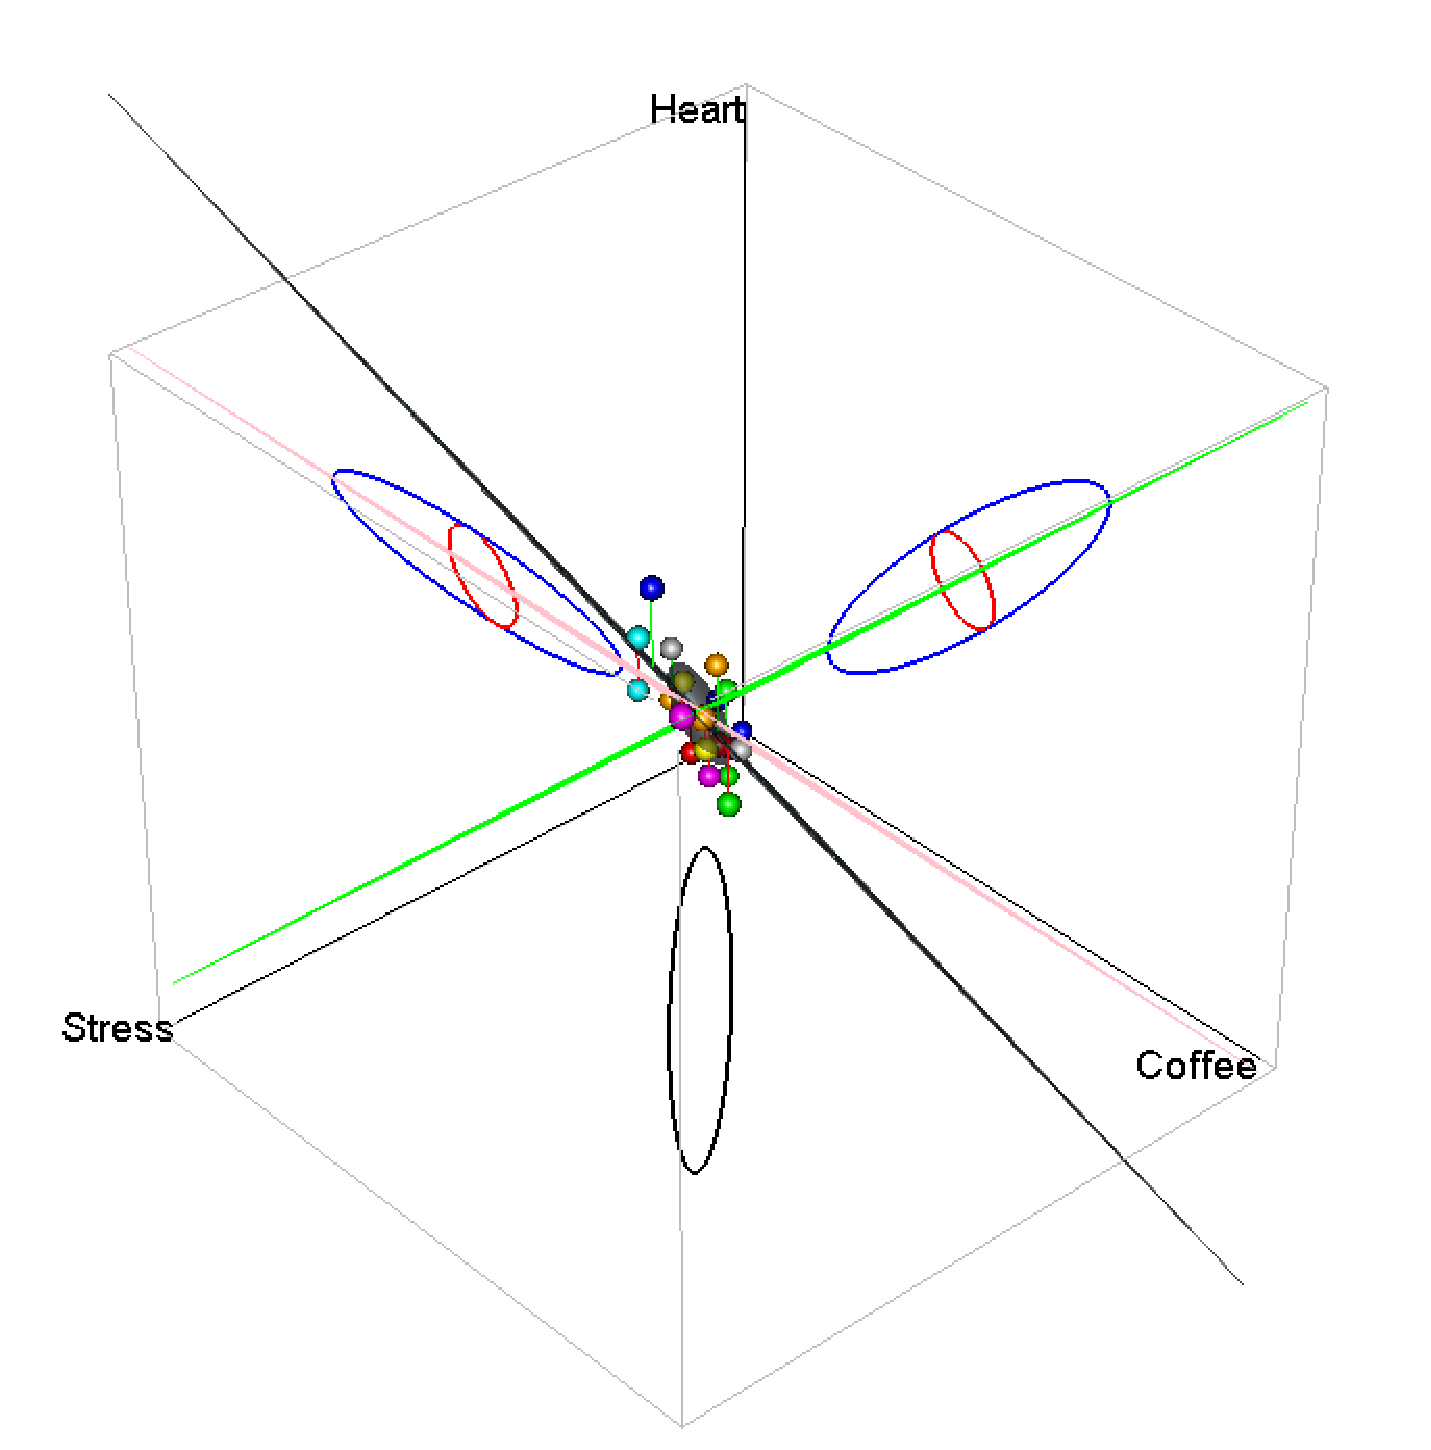
\includegraphics[width=1\linewidth]{fig/coffee-av3D-2}
 \end{minipage}
  \caption{3D views of the relationship between Heart, Coffee and Stress, showing the three regression planes
  for the marginal models, Heart $\sim$ Coffee (green), Heart $\sim$ Stress (pink), and the joint model, Heart $\sim$ Coffee $+$ Stress (light blue).
  Left: a standard view; right: a view showing all three regression planes on edge.
  The ellipses in the side panels are 2D projections of the standard conditional (red) and marginal (blue) ellipsoids, as shown in \figref{fig:coffee-avplot-B}.
  }
  \label{fig:coffee-av3D}
\end{figure}

%For three variables, $(y, x_1, x_2)$, the added variable plot for, say $x_1$, has particularly simple geometric interpretations in 3D in terms
%of the fitted planes for the full model, $y \sim x_1 + x_2$, the marginal model, $y \sim  x_2$

\figref{fig:coffee-avplot-A} shows added-variable plots for Stress and Coffee in the multiple regression predicting Heart disease,
supplemented by data ellipses for the residuals $(\vec{x}_k^\star, \vec{y}^\star)$.  With reference to the properties
of data ellipses in marginal scatterplots (see \figref{fig:ellipses-demo}), the following visual properties (among others)
are useful in this discussion.  These results follow simply from translating ``marginal'' into ``conditional'' (or ``partial'')
in the present context. 
The essential idea is that the data ellipse of the AVP for $(x_k, y)$ is to the estimate of a coefficient in a multiple regression as
 the data ellipse of $(x, y)$ is to simple regression. Thus:


\begin{figure}[htb]
 \begin{minipage}[b]{.49\linewidth}
  \centering
  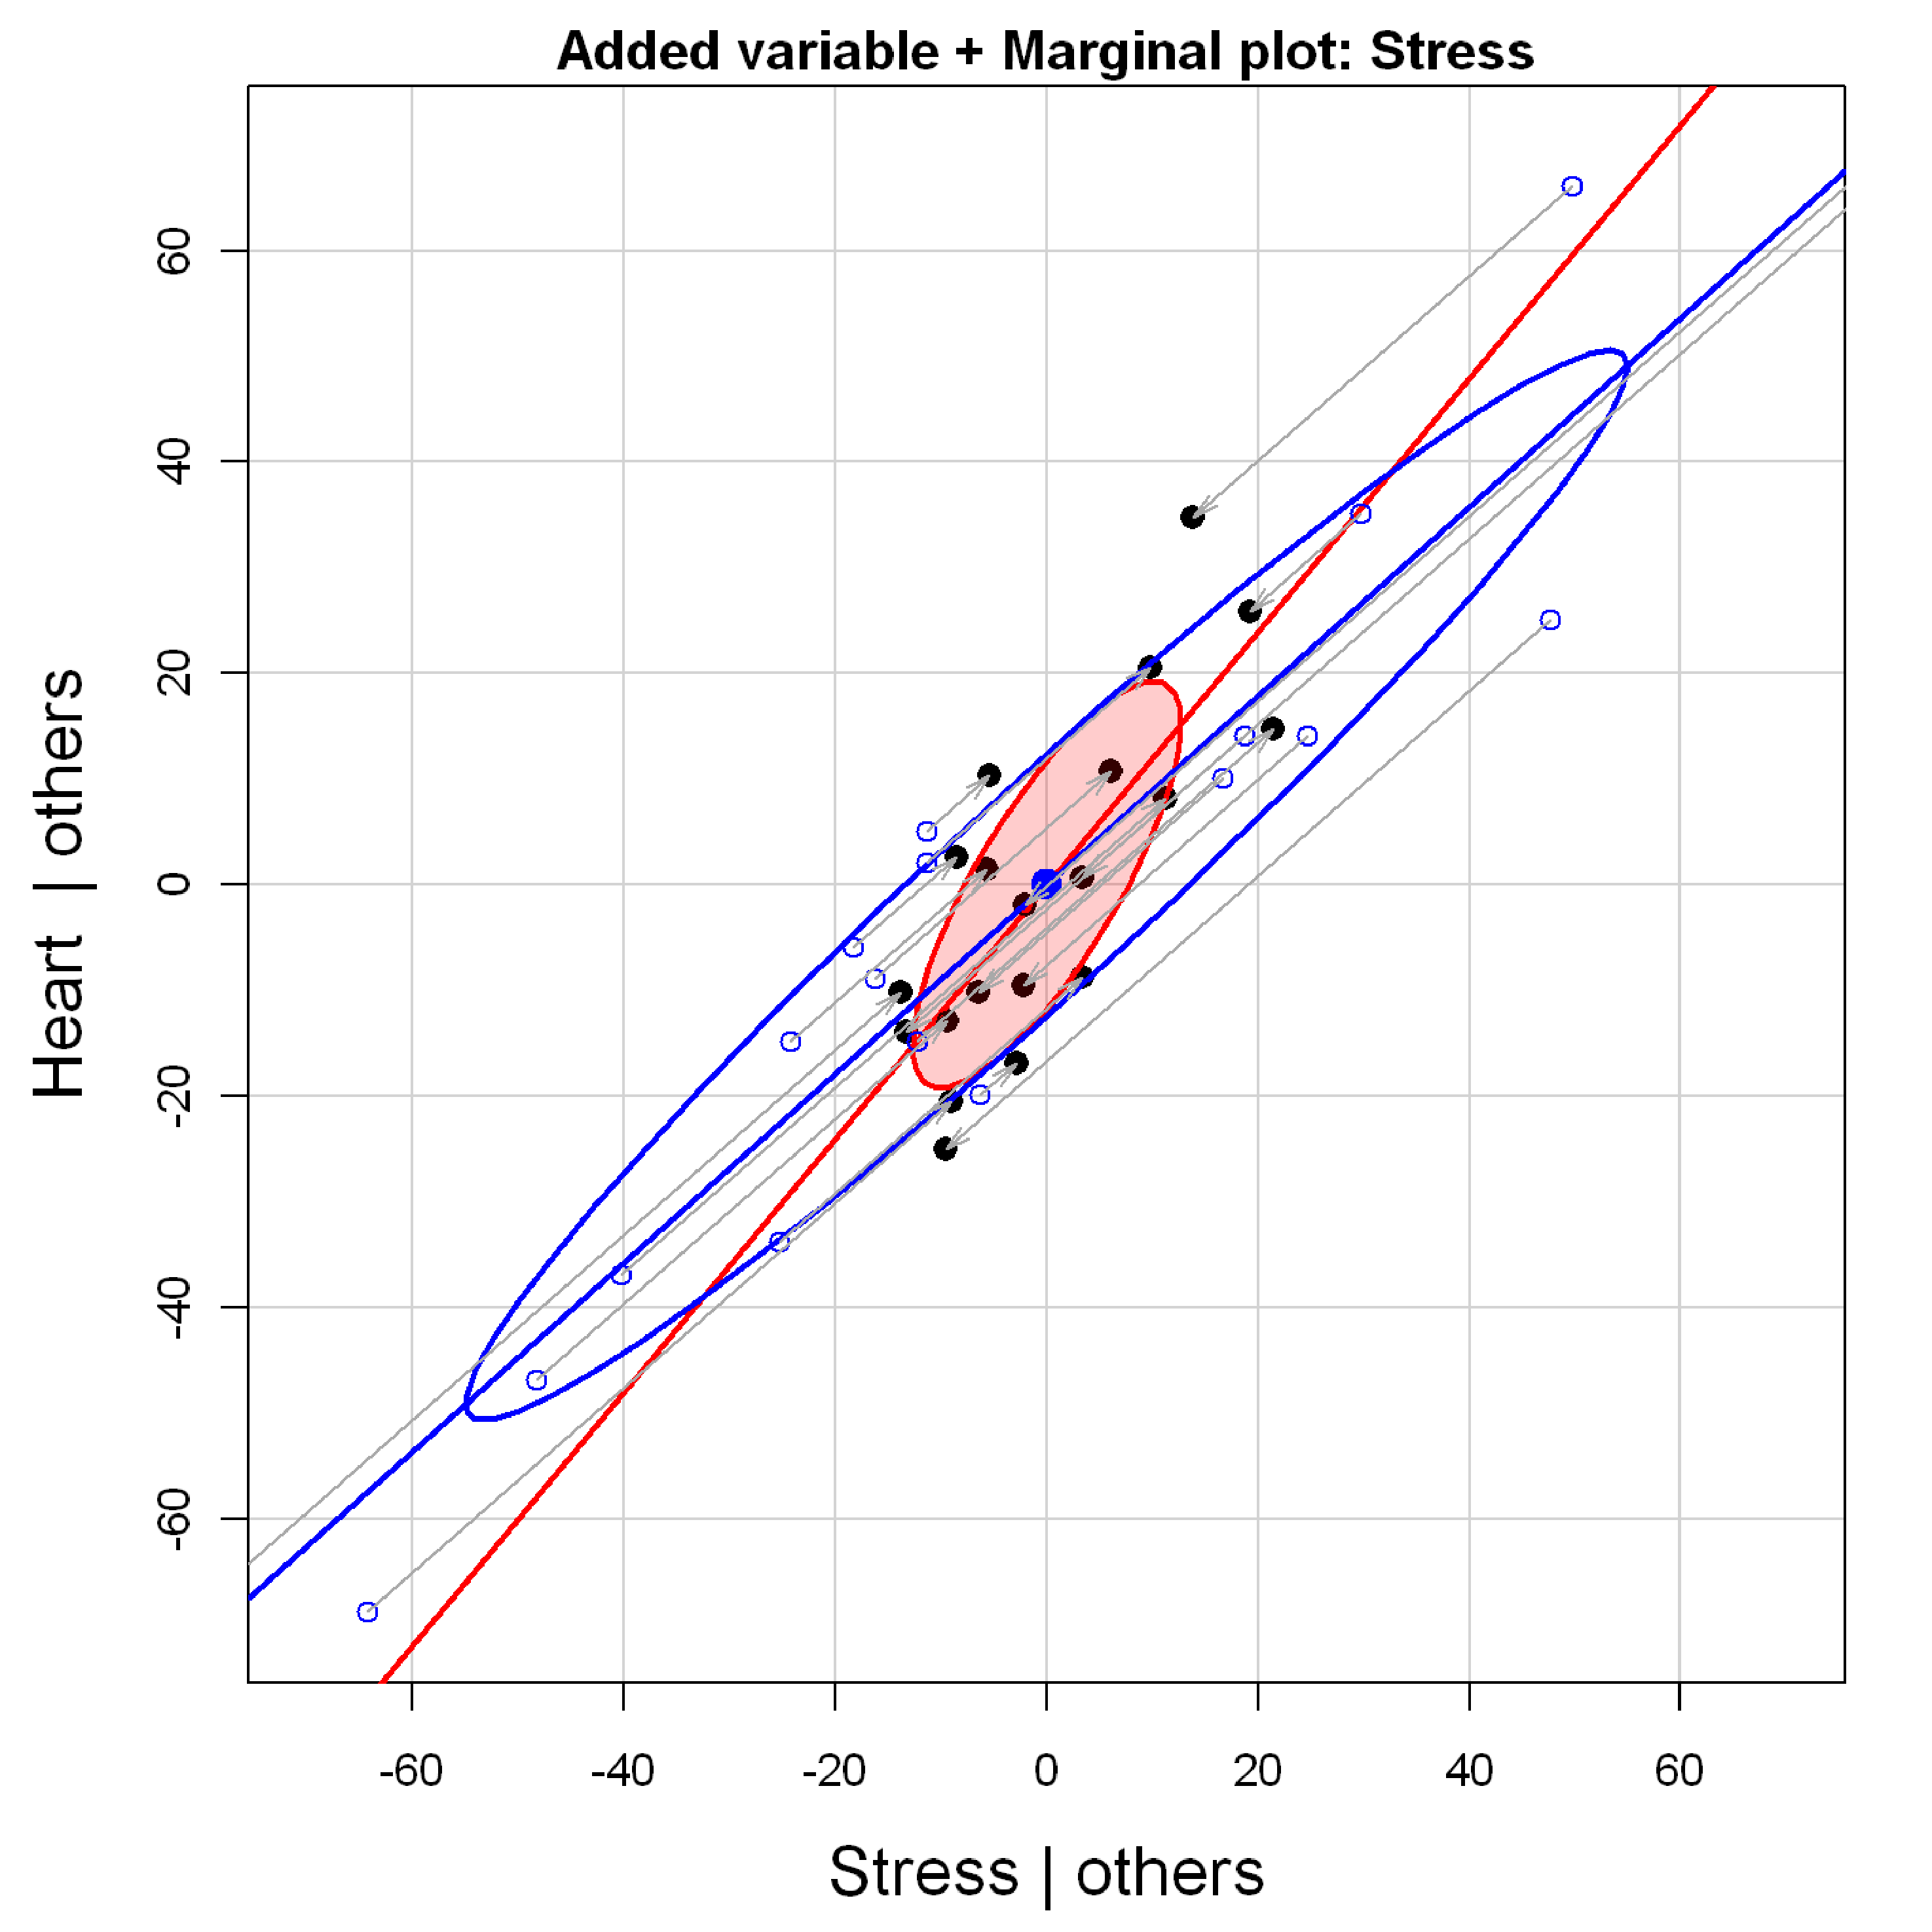
\includegraphics[width=1\linewidth]{fig/coffee-avplot3}
%  \caption{}%
%  \label{fig:}
 \end{minipage}%
 \hfill
 \begin{minipage}[b]{.49\linewidth}
  \centering
  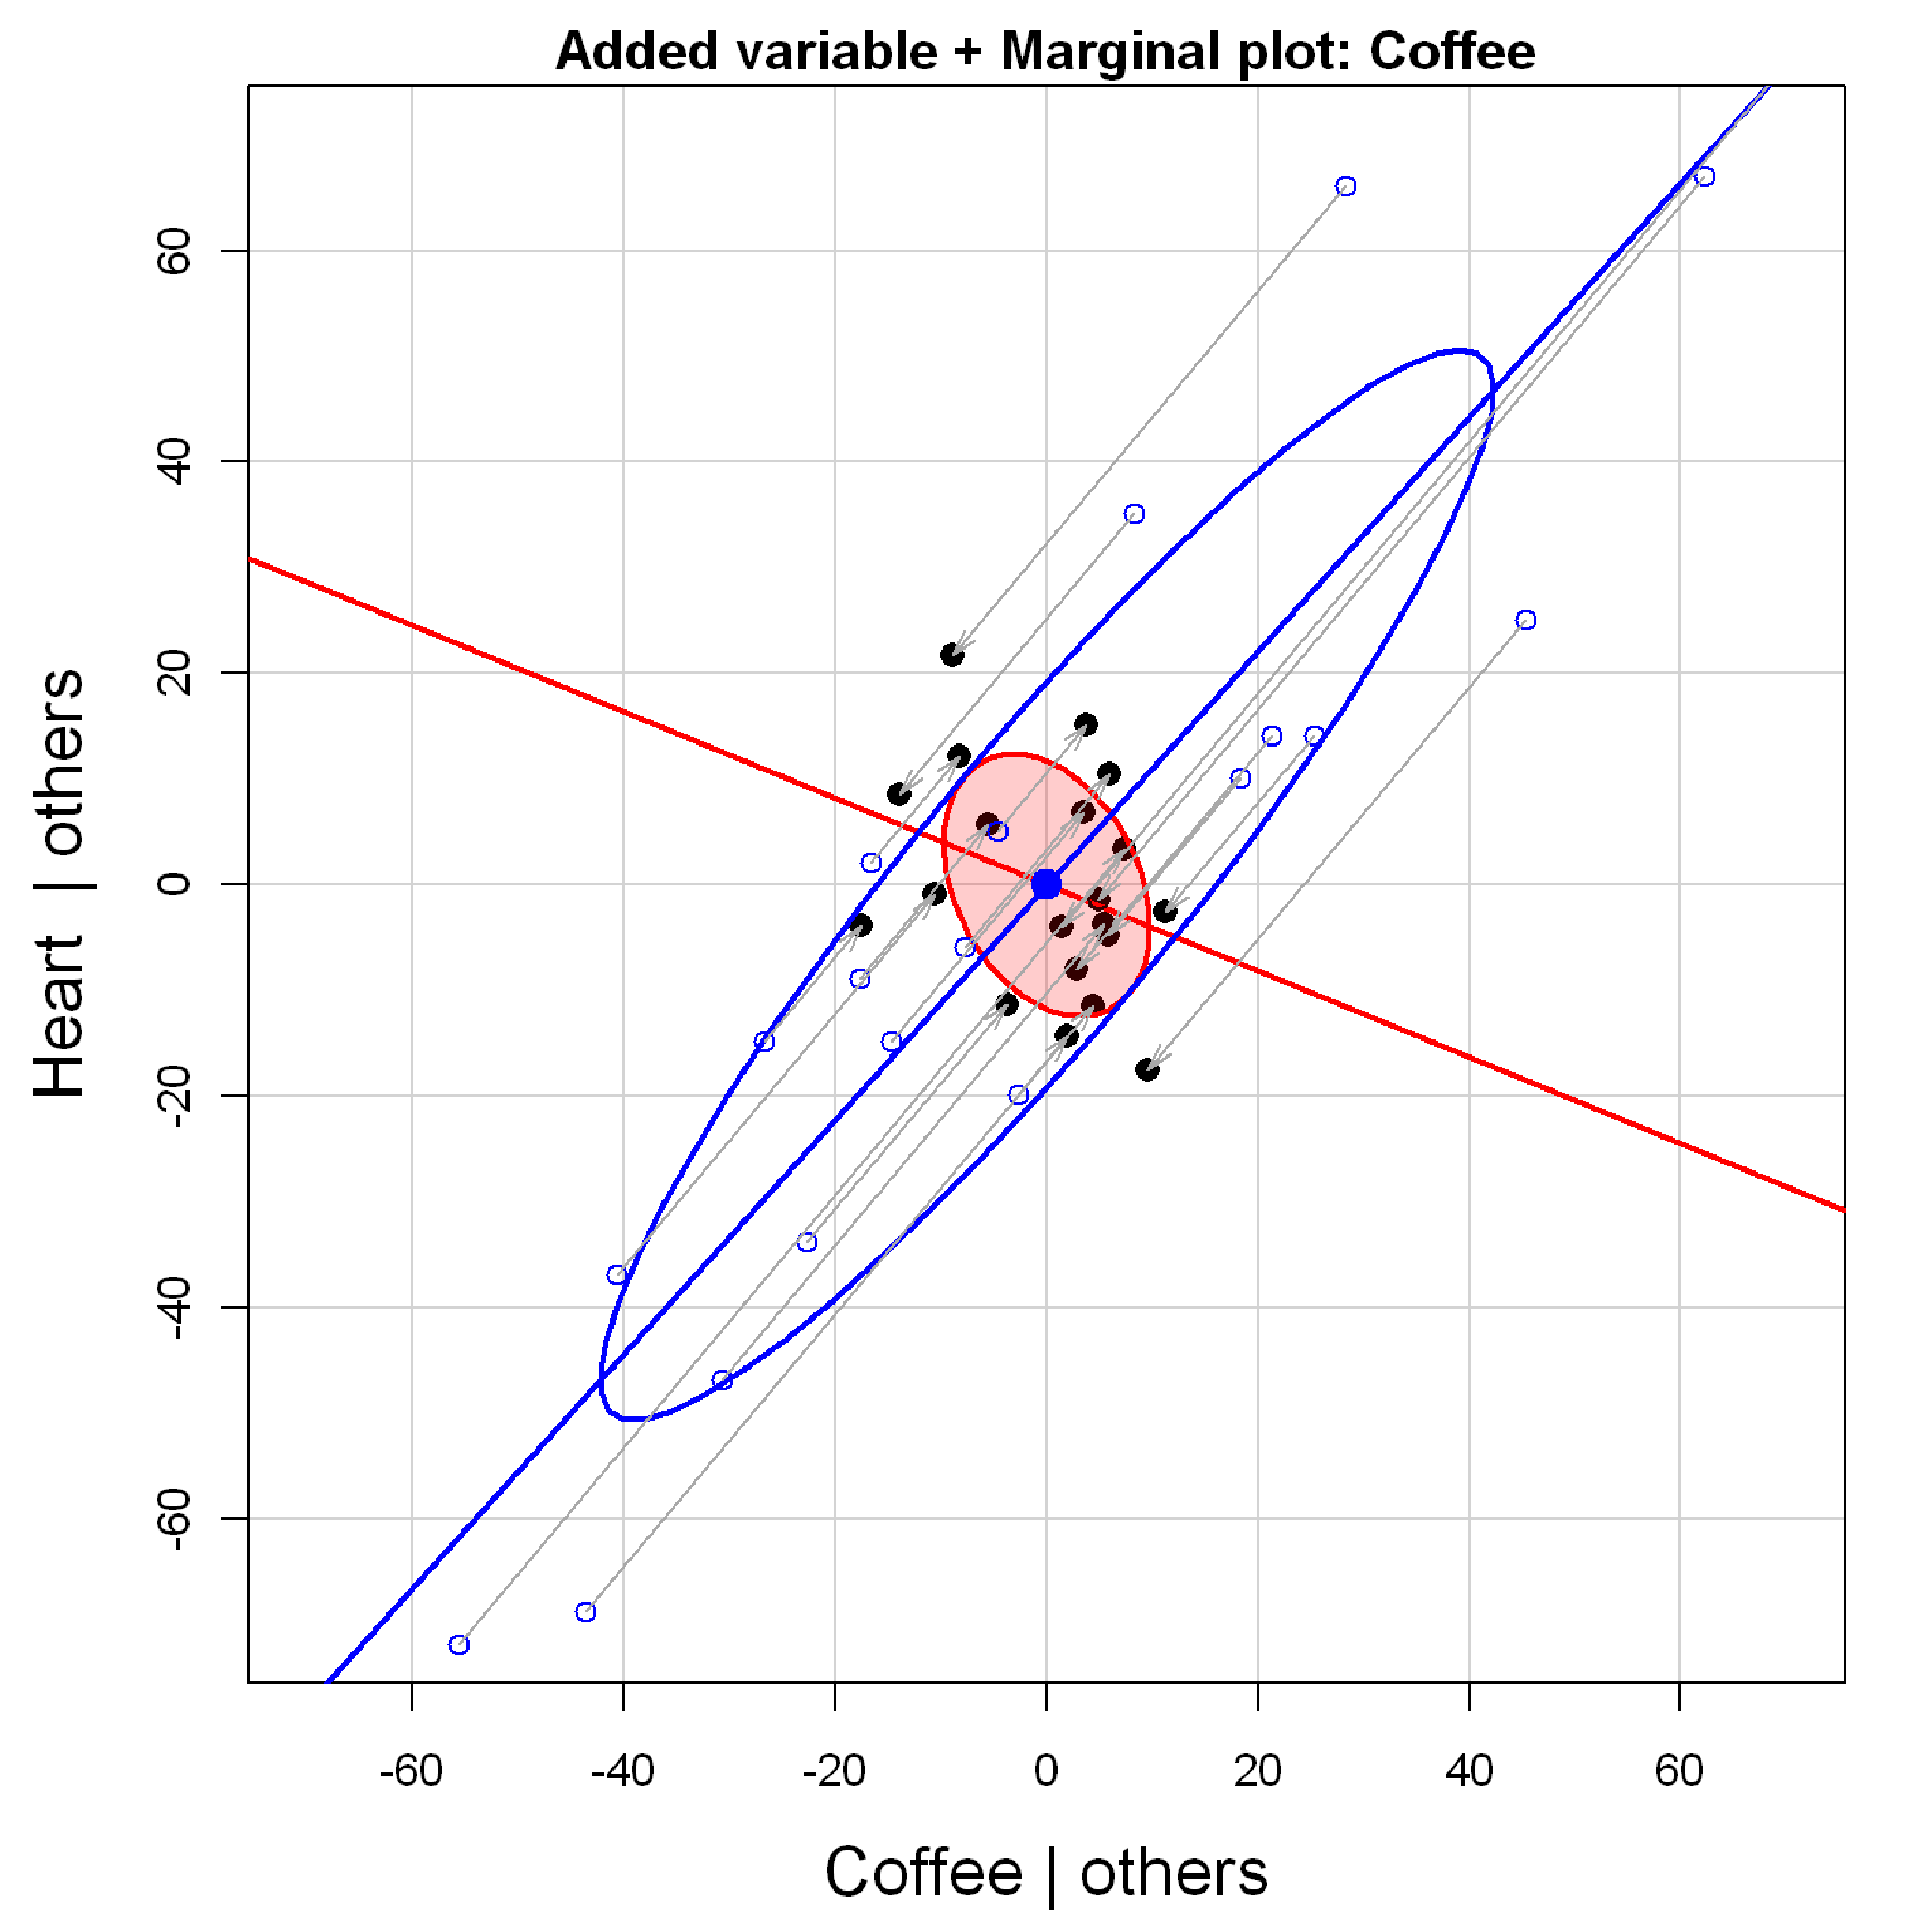
\includegraphics[width=1\linewidth]{fig/coffee-avplot4}
 \end{minipage}
  \caption{Added-variable $+$ marginal plots for Stress and Coffee in the multiple regression predicting Heart disease.
Each panel shows the 50\% conditional data ellipse for $x^{*}, y^{*}$ residuals (shaded, red) as well as the marginal 50\%
data ellipse for the $(x, y)$ variables, shifted to the origin.
Arrows connect the mean-centered marginal points (open circles) to the residual points (filled circles).}
  \label{fig:coffee-avplot-B}
\end{figure}

\begin{enumerate*}
%  \item The data ellipse of the AVP for $(x_k, y)$ is to the estimate of a coefficient in a multiple regression as
%  the data ellipse of $(x, y)$ is to simple regression. Thus:

 \item The simple regression least squares fit of $\vec{y}^\star$ on $\vec{x}_k^\star$ has slope $\hat{\beta_k}$,
 the partial slope for $x_k$ in the full model (and intercept = 0).

 \item The residuals, $(\vec{y}^\star - \widehat{\vec{y}}^\star)$, shown in this plot are the residuals for $\vec{y}$ in the full model.

 \item The correlation between $\vec{x}_k^\star$ and $\vec{y}^\star$, seen in the shape of the data ellipse for these residuals,
 is the partial correlation between $y$ and $x_k$ with the other predictors in $\mat{X}_{[-k]}$ partialled out.

 \item The horizontal half-width of the AVP data ellipse is proportional to the conditional standard deviation of
 $x_k$ remaining after all other predictors have been accounted for, providing a visual interpretation
 of variance inflation due to collinear predictors, as we describe below.

 \item The vertical half-width of the data ellipse is proportional to the residual standard deviation $s_e$ in the multiple regression.

 \item The squared horizontal positions, $(\vec{x}_k^\star)^2$, in the plot give the partial contributions
 to leverage on the coefficient $\hat{\beta}_k$ of $x_k$. 

 \item Items (3) and (7) imply that 
 that the AVP for $x_k$ shows the \emph{partial} influence of individual observations on the coefficient $\hat{\beta}_k$, 
 in the same way as in \figref{fig:levdemo21} for marginal models. These influence statistics are
 often shown numerically
 as DFBETA statistics \citep{Belsley-etal:80}.
 
 \item The last three items imply that the collection of added-variable plots for $\vec{y}$ and
 $\mat{X}$ provide an easy way to visualize the influence that individual observations---and indeed the joint influence of subsets of observations---have on
 the esimation of \emph{each} coefficient in a given model.
\end{enumerate*}


Elliptical insight also permits us to go further, to depict the relationship between conditional and marginal views
directly.
\figref{fig:coffee-avplot-B} shows the same added-variable plots for Heart disease on Stress and Coffee
as in \figref{fig:coffee-avplot-A} (with a zoomed-out scaling), but here we also overlay the
marginal data ellipses for $(x, y)$,
and and marginal regression lines for Stress and Coffee separately.  In 3D data space,
these are the shadows (projections) of the data ellipsoid onto the planes defined by the
partial variables.  In 2D AVP space, these are just the marginal data ellipses translated to
the origin.

The most obvious feature of \figref{fig:coffee-avplot-B} is that the AVP for Coffee has a negative slope in the conditional
plot (suggesting that controlling for Stress, coffee consumption is good for your heart), while
in the marginal plot increasing coffee seems to be bad for your heart. This serves as a
regression example of Simpson's paradox, which we considered earlier.

Less obvious is the fact that
the marginal and AVP ellipses are easily visualized as a shadow versus a slice of the full data ellipsoid.
Thus, the AVP ellipse must be contained in the marginal ellipse, as we can see in \figref{fig:coffee-avplot-B}.
If there are only two $x$s, then the AVP ellipse must touch the marginal ellipse at two points.
% This implies interesting contraints among the three quantities: improvement in fit, VIF, and change from marginal to conditional slope.
The shrinkage of the intersection of the AVP ellipse with the $y$ axis represents improvement in fit due to other $x$s.

More importantly, the shrinkage of the width (projected onto a horizontal axis) represents the
square root of the variance inflation factor (VIF), which can be shown to be the ratio of the horizontal
width of the marginal ellipse of $(x_k, y)$, with standard deviation $s(x_k)$ to the width of the conditional
ellipse of $(x_k^\star, y^\star)$, with standard deviation $s(x_k \given \textrm{others})$.
This geometry implies interesting contraints among the three quantities: improvement in fit, VIF, and change from the marginal to conditional slope.

Finally, \figref{fig:coffee-avplot-B} also shows how conditioning on other predictors works for individual
observations, where each point of  $(\vec{x}_k^\star, \vec{y}^\star)$ is the image of $(\vec{x}_k, \vec{y})$
along the path of the marginal regression. This reminds us that the AVP is a 2D projection of the full space,
where the regression plane of $\vec{y}$ on $\mat{X}_{[-k]}$ becomes the vertical axis and
the regression plane of $\vec{x}_k$ on $\mat{X}_{[-k]}$ becomes the horizontal axis.

